% Created 2023-07-12 Wed 15:38
% Intended LaTeX compiler: xelatex
\documentclass[11pt,twoside,twocolumn,landscape]{article}
\usepackage{graphicx}
\usepackage{longtable}
\usepackage{wrapfig}
\usepackage{rotating}
\usepackage[normalem]{ulem}
\usepackage{amsmath}
\usepackage{amssymb}
\usepackage{capt-of}
\usepackage{hyperref}
\usepackage{subcaption}
\usepackage[newfloat]{minted}
\usepackage{color}
\usepackage{listings}
\usepackage[top=2cm,bottom=2cm,right=2cm,left=2cm,landscape]{geometry}
\usepackage{multicol}
\usepackage{enumitem}
\usepackage{fancyhdr}
\usepackage{caption}
\usepackage{algorithm}
\usepackage{algpseudocode}
\usepackage{float}
\setlist[description]{itemsep=-1pt,leftmargin=2mm,topsep=0pt}
\setlist[itemize]{itemsep=-1pt,topsep=0pt}
\setlist{noitemsep}
\setlength{\parindent}{0pt}
\setlength{\columnseprule}{0.2pt}
\definecolor{mygreen}{rgb}{0,0.6,0}
\definecolor{mygray}{rgb}{0.5,0.5,0.5}
\definecolor{mymauve}{rgb}{0.58,0,0.82}
\lstset{ backgroundcolor=\color{white}, basicstyle=\footnotesize, breaklines=true, captionpos=b, commentstyle=\color{mygreen}, escapeinside={\%*}{*)},keywordstyle=\color{blue}, stringstyle=\color{mymauve},}
\usepackage{caption}
\author{Olivier Lischer}
\date{\today}
\title{CPlA API}
\hypersetup{
 pdfauthor={Olivier Lischer},
 pdftitle={CPlA API},
 pdfkeywords={},
 pdfsubject={},
 pdfcreator={Emacs 28.2 (Org mode 9.7-pre)}, 
 pdflang={English}}
\begin{document}

\pagestyle{fancy}
\fancyhf{}
\fancyhead[R]{CPlA-FS23}
\fancyhead[L]{Exam Summary}
\fancyfoot[CE,CO]{\leftmark}
\fancyfoot[R]{\thepage}
\fancyfoot[L]{Olivier Lischer}


\section{Type Traits}
\label{sec:org45db718}

\begin{center}
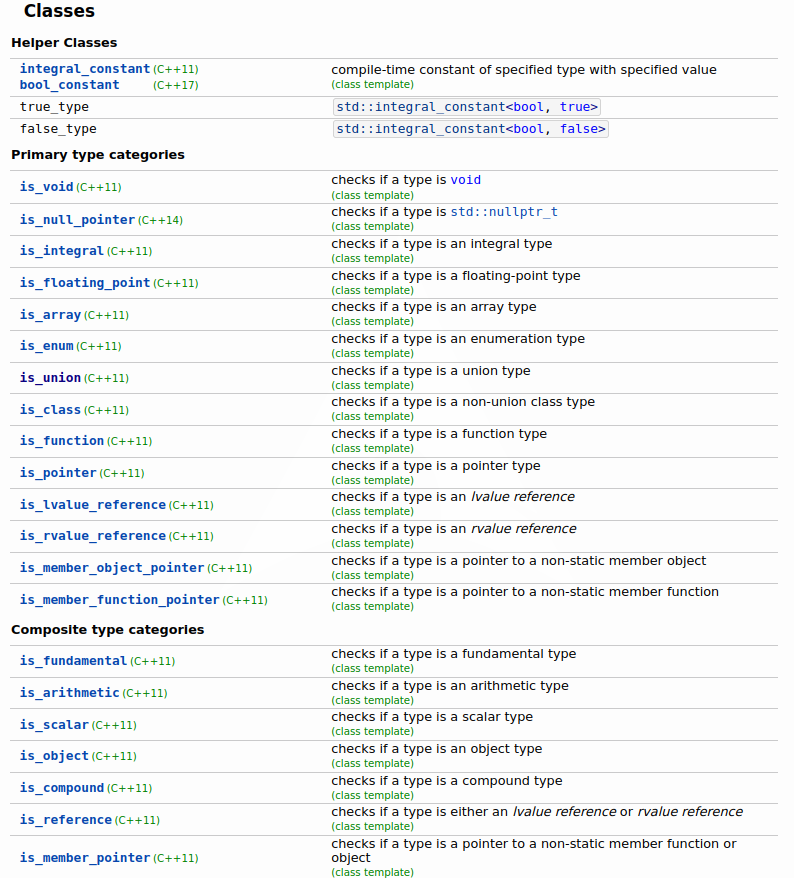
\includegraphics[width=.9\linewidth]{img/type_traits_1.png}
\end{center}
\begin{center}
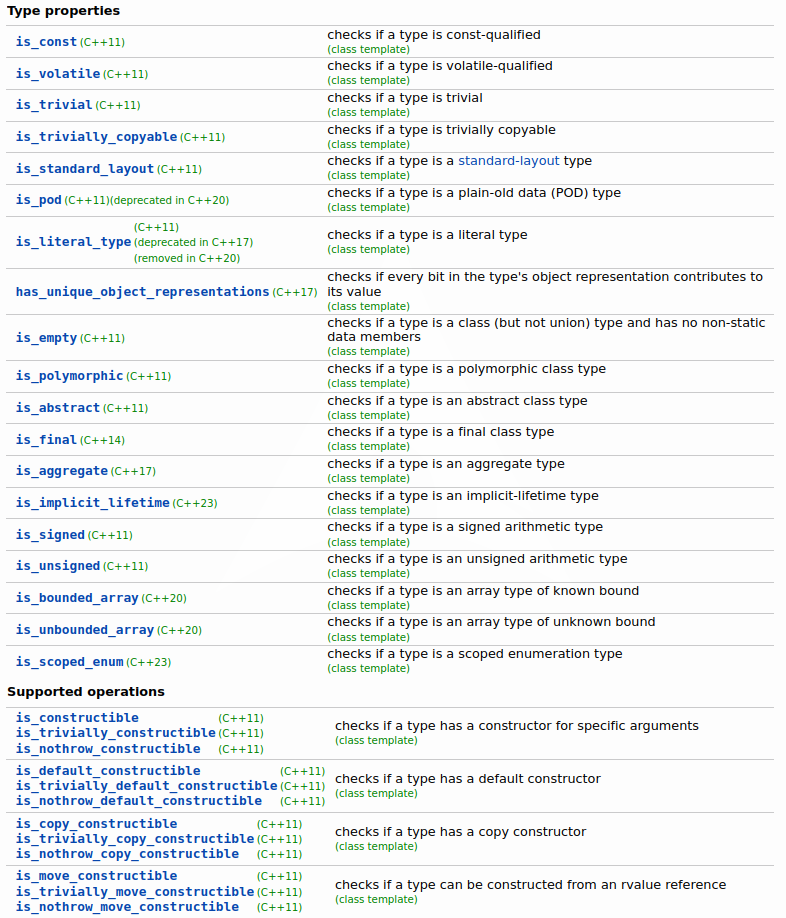
\includegraphics[width=.9\linewidth]{img/type_traits_2.png}
\end{center}
\begin{center}
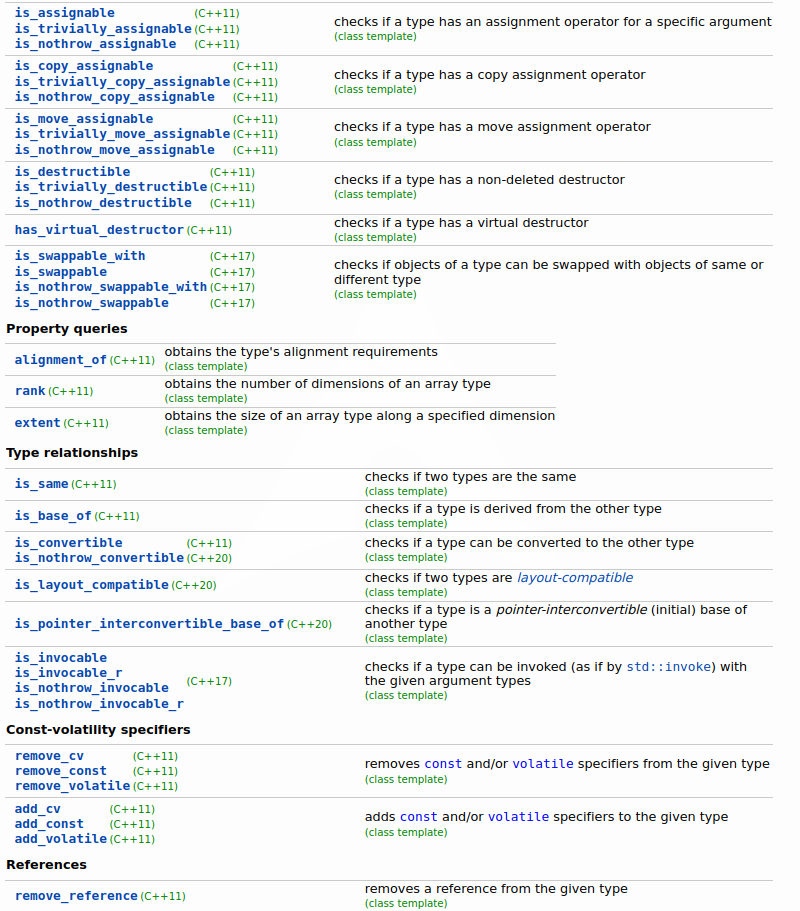
\includegraphics[width=.9\linewidth]{img/type_traits_3.png}
\end{center}
\begin{center}
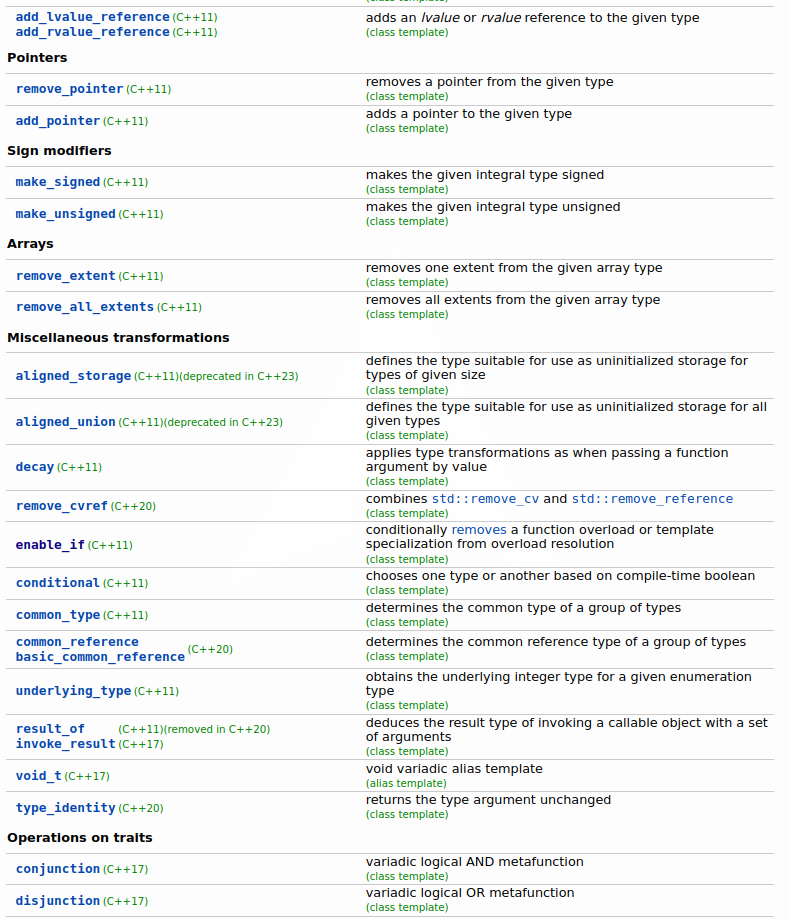
\includegraphics[width=.9\linewidth]{img/type_traits_4.png}
\end{center}
\begin{center}
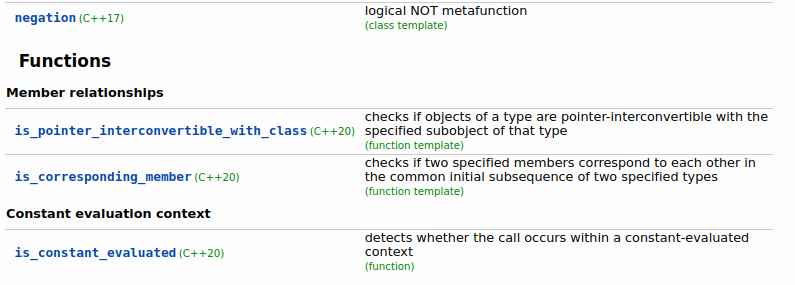
\includegraphics[width=.9\linewidth]{img/type_traits_5.png}
\end{center}
\end{document}